\subsection{Introduction}

\begin{frame}{LoRaWAN}
\framesubtitle{Introduction}
\begin{center}
\scalebox{0.8}{%
\begin{tikzpicture}[auto,node distance=1.2cm]
  \tikzstyle{comment}=[ right=2pt, font=\small, fill=white, text=black, draw=black, ]
  \tikzstyle{every state}=[rectangle,thick,draw=black,fill=gray!20,text=black, minimum width= 6cm, minimum height= 1.00cm ]
  \tikzstyle{smallstate}=[rectangle,thick,draw=black!80,fill=gray!10,text=black, minimum width= 6cm, minimum height= 0.25cm ]
  \tikzstyle{innerstate}=[rectangle,thick,draw=black,fill=gray!10,text=black, minimum width= 4cm, minimum height= 1.00cm ]

  \node[state,color=gray!40,fill=gray!20] at (0, 0) (A)            { Application Layer};
  \node[state,color=gray!40,fill=gray!20]         (E) [below of=A] { Network Layer};
  \node[state]         (F) [below of=E]                            { LoRaWAN };
  \node[state]         (G) [below of=F]                            { LoRa };

  \node[comment]       at (F.north west) {MAC Layer};
  \node[comment]       at (G.north west) {Physical Layer};
\end{tikzpicture}
}
\end{center}

\end{frame}

\subsection{LoRaWAN ?}

\begin{frame}{LoRaWAN}
\framesubtitle{Organisation de LoRaWAN}
% Photo gateway + schema organisation
\begin{columns}
  \begin{column}{0.5\textwidth}
    \begin{itemize}
      \item Écoute sur toutes les fréquences/SF
      \item Envoie les messages sur un serveur
      \item Application récupères les données à l'aide d'une API
    \end{itemize}
    \makebox[\linewidth]{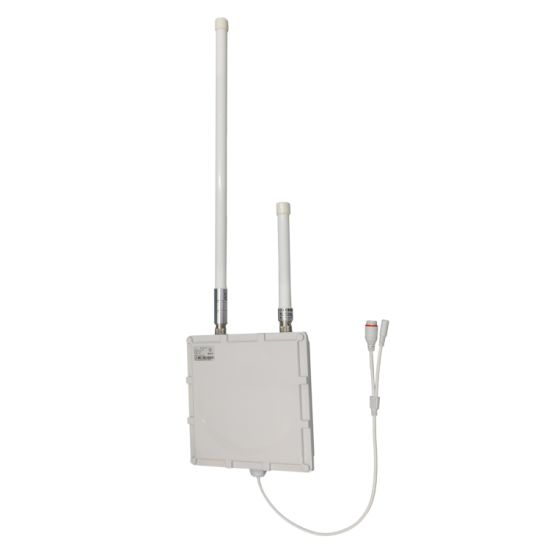
\includegraphics[page=1,width=0.3\paperwidth]{presentation.tex/fig/gateway.jpg}}
  \end{column}
  \begin{column}{0.5\textwidth}
    \begin{center}
\scalebox{0.6}{
\begin{tikzpicture}[
  radiation/.style={{decorate,decoration={expanding waves,angle=90,segment length=4pt}}},
  ports/.style={
    line width=0.3pt,
    top color=gray!20,
    bottom color=gray!80
  },
  rack switch/.style={
    minimum width=1.25cm,
    minimum height=0.25cm,
    parallelepiped,fill=white, draw,
    parallelepiped offset x=2mm,
    parallelepiped offset y=1.25mm,
    xscale=-1,
    path picture={
      \draw[top color=gray!5,bottom color=gray!40]
      (path picture bounding box.south west) rectangle
      (path picture bounding box.north east);
      \coordinate (A-west) at ([xshift=-0.2cm]path picture bounding box.west);
      \coordinate (A-center) at ($(path picture bounding box.center)!0!(path
        picture bounding box.south)$);
      \foreach \x in {0.275,0.525,0.775}{
        \draw[ports]([yshift=-0.05cm]$(A-west)!\x!(A-center)$)
          rectangle +(0.1,0.05);
        \draw[ports]([yshift=-0.125cm]$(A-west)!\x!(A-center)$)
          rectangle +(0.1,0.05);
       }
      \coordinate (A-east) at (path picture bounding box.east);
      \foreach \x in {0.085,0.21,0.335,0.455,0.635,0.755,0.875,1}{
        \draw[ports]([yshift=-0.1125cm]$(A-east)!\x!(A-center)$)
          rectangle +(0.05,0.1);
      }
    }
  },
  server/.style={
    fill=white, draw,
    minimum width=0.35cm,
    minimum height=0.75cm,
    parallelepiped,
    parallelepiped offset x=3mm,
    parallelepiped offset y=2mm,
    xscale=-1,
    path picture={
      \draw[top color=gray!5,bottom color=gray!40]
      (path picture bounding box.south west) rectangle
      (path picture bounding box.north east);
      \coordinate (A-center) at ($(path picture bounding box.center)!0!(path
        picture bounding box.south)$);
      \coordinate (A-west) at ([xshift=-0.575cm]path picture bounding box.west);
      \draw[ports]([yshift=0.1cm]$(A-west)!0!(A-center)$)
        rectangle +(0.2,0.065);
      \draw[ports]([yshift=0.01cm]$(A-west)!0.085!(A-center)$)
        rectangle +(0.15,0.05);
      \fill[black]([yshift=-0.35cm]$(A-west)!-0.1!(A-center)$)
        rectangle +(0.235,0.0175);
      \fill[black]([yshift=-0.385cm]$(A-west)!-0.1!(A-center)$)
        rectangle +(0.235,0.0175);
      \fill[black]([yshift=-0.42cm]$(A-west)!-0.1!(A-center)$)
        rectangle +(0.235,0.0175);
    }
  },
  antenna/.pic={
    code={\tikzset{scale=2/10}
      \draw[semithick] (0,0) -- (1,4);% left line
      \draw[semithick] (3,0) -- (2,4);% right line
      \draw[semithick] (0,0) arc (180:0:1.5 and -0.5);
      \node[inner sep=4pt] (circ) at (1.5,5.5) {};
      \draw[semithick] (1.5,5.5) circle(8pt);
      \draw[semithick] (1.5,5.5cm-8pt) -- (1.5,4);
      \draw[semithick] (1.5,4) ellipse (0.5 and 0.166);
      \draw[semithick,radiation,decoration={angle=45}] (1.5cm+8pt,5.5) -- +(0:2);
      \draw[semithick,radiation,decoration={angle=45}] (1.5cm-8pt,5.5) -- +(180:2);
    }
  },
  node/.pic={
    code={\tikzset{scale=2/10}
      \draw[semithick] (1.5,-0.5) -- (1.5,1.5cm-8pt);
      \draw[semithick] (1.5,1.5) circle(8pt);
      \draw[semithick,radiation,decoration={angle=45}] (1.5cm+8pt,1.5) -- +(0:3);
      \draw[semithick,radiation,decoration={angle=45}] (1.5cm-8pt,1.5) -- +(180:3);
    }
  }
]
  \draw[color=blue!20,fill=blue!20] (-1.8,2) circle (2.8cm);
  \draw[color=blue!20,fill=blue!20] (-1.8,0) circle (2.3cm);
  \draw[color=blue!20,fill=blue!20] (-1.8,-2) circle (2.8cm);

  \path (0.5,0) edge [-,semithick,draw=gray!70] (2,0);
  \path (2,0) edge [-,semithick,draw=gray!70] (4,2);
  \path (2,0) edge [-,semithick,draw=gray!70] (4,0);
  \path (2,0) edge [-,semithick,draw=gray!70] (4,-2);

  \path (0,-0.4) pic [fill=white,scale=1] {antenna};

  \path (-2,2) pic [black,scale=0.8] {node};
  \path (-2,0) pic [black,scale=0.8] {node};
  \path (-2,-2) pic [black,scale=0.8] {node};

  \node[rack switch] at (2,0) {};

  \node[server] (loraserv) at (4,0) {};
  \node[server] (loraserv) at (4,2) {};
  \node[server] (loraserv) at (4,-2) {};
\end{tikzpicture}
}
\end{center}
 
    
  \end{column}
\end{columns}
\end{frame}

\begin{frame}{LoRaWAN}
\framesubtitle{Un protocole MAC ?}

\begin{block}{MAC}
Elle sert d'interface entre la partie logicielle contrôlant la 
liaison d'un nœud (Contrôle de la liaison logique) et la couche 
physique (matérielle). Par conséquent, elle est différente selon 
le type de média physique utilisé (Ethernet, WLAN, …)
\end{block}

\end{frame}

\begin{frame}{LoRaWAN}
\framesubtitle{Aloha}
\begin{block}{}
{
  Quel moyen le plus simple d'interfacer la couche physique ?
}
\end{block}
\begin{columns}
\begin{column}{0.5\textwidth}
\begin{center}
\scalebox{0.7}{
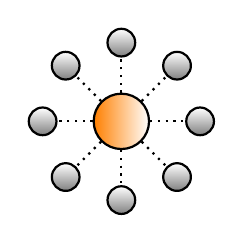
\begin{tikzpicture}[auto, thick]
    \tikzstyle{motes}=[draw,circle,bottom color= gray,
                      top color= white,minimum width=10pt]
    \tikzstyle{gateways}=[draw,circle, left color= orange,minimum width=20pt]
    \foreach \place/\name in {{(0,0)/a}}
        \node[gateways] (\name) at \place {};
    % Place normal peers
    \foreach \pos/\i in {below left of/1, below of/2, left of/3, above left of/4, below right of/5,above of/6, right of/7, above right of/8}
        \node[motes, \pos =a ] (a\i) {};
    \foreach \speer/\peer in {a/a1,a/a2,a/a3,a/a4,a/a5,a/a6,a/a7,a/a8}
        \path[dotted] (\speer) edge (\peer);
\end{tikzpicture}
}
\end{center}
\begin{center}
\scalebox{0.5}{%
\begin{tabular}{r@{ }l r@{ }l}

\begin{tikzpicture}\draw[left color=orange,line width=1pt] circle(1ex);\end{tikzpicture} & Gateway & 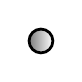
\begin{tikzpicture}\draw[left color=gray,line width=1pt] circle(1ex);\end{tikzpicture} & Mote
\end{tabular}
}
\end{center}
\end{column}
\begin{column}{0.5\textwidth}
\begin{center}
  \scalebox{0.6}{
  \begin{tikzpicture}[
    ack/.style={draw, rectangle, fill=orange!40, inner sep=0pt, outer sep=0pt},
    tx/.style={draw, rectangle, fill=blue!30,inner sep=0pt, outer sep=0pt},
    relay/.style={draw, rectangle, fill=green!30,inner sep=0pt, outer sep=0pt},
    rx/.style={draw, pattern=north west lines, pattern color=black!60, rectangle, inner sep=0pt, outer sep=0pt},
    arr/.style={help lines,black!70,<->},
    ]
    \draw[->,thick] (-0.1,0)--(6,0) node[right]{time};
    \draw[->,thick] (0,-0.1)--(0,4) node[above]{};

    \draw[dotted] (-0.1,0.5)--(6,0.5);
    \node[] at (-1.2, 1) {Gateway};
    \draw[] (-0.1,1)--(0.1,1);
    \draw[dotted] (-0.1,1.5)--(6,1.5);
    \node[] at (-1.2, 2) {Node 1};
    \draw[] (-0.1,2)--(0.1,2);
    \draw[dotted] (-0.1,2.5)--(6,2.5);
    \node[] at (-1.2, 3) {Node 2};
    \draw[] (-0.1,3)--(0.1,3);
    \draw[dotted] (-0.1,3.5)--(6,3.5);

    % Gateway
    \node () [rx, fit={(0.1,0.7) (5.9,1.3)}] {};
    % Relay
    \node () [tx, fit={(1.1,1.7) (1.4,2.3)}] {};
    \node () [tx, fit={(3.1,1.7) (3.4,2.3)}] {};
    \node () [tx, fit={(5.1,1.7) (5.4,2.3)}] {};
    % Node
    \node () [tx, fit={(2.1,2.7) (2.4,3.3)}] {};
    \node () [tx, fit={(5.1,2.7) (5.4,3.3)}] {};
  \end{tikzpicture}
  }
  % \caption{Collision between nodes}
  \scalebox{0.6}{
  \begin{tabular}{r@{ }l r@{ }l}
  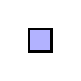
\begin{tikzpicture}\draw[fill=blue!30,line width=1pt] +(-4pt,-4pt) rectangle +(4pt,4pt);\end{tikzpicture} & Transmission 
    & \begin{tikzpicture}\draw[pattern=north west lines, pattern color=black!90,line width=1pt] +(-4pt,-4pt) rectangle +(4pt,4pt);\end{tikzpicture} & Reception
  \end{tabular}
  }
\end{center}
\end{column}
\end{columns}

\end{frame}

\begin{frame}{LoRaWAN}
\framesubtitle{Acknowledgement}
\begin{block}{}
{
  Comment s'assurer de la récèption du message ?
}
\end{block}
\begin{columns}
\begin{column}{0.4\textwidth}
\begin{center}
\scalebox{0.7}{
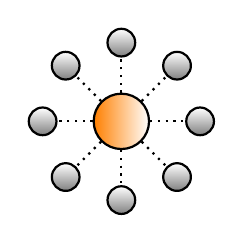
\begin{tikzpicture}[auto, thick]
    \tikzstyle{motes}=[draw,circle,bottom color= gray,
                      top color= white,minimum width=10pt]
    \tikzstyle{gateways}=[draw,circle, left color= orange,minimum width=20pt]
    \foreach \place/\name in {{(0,0)/a}}
        \node[gateways] (\name) at \place {};
    % Place normal peers
    \foreach \pos/\i in {below left of/1, below of/2, left of/3, above left of/4, below right of/5,above of/6, right of/7, above right of/8}
        \node[motes, \pos =a ] (a\i) {};
    \foreach \speer/\peer in {a/a1,a/a2,a/a3,a/a4,a/a5,a/a6,a/a7,a/a8}
        \path[dotted] (\speer) edge (\peer);
\end{tikzpicture}
}
\end{center}
\begin{center}
\scalebox{0.6}{%
\begin{tabular}{r@{ }l r@{ }l}

\begin{tikzpicture}\draw[left color=orange,line width=1pt] circle(1ex);\end{tikzpicture} & Gateway & 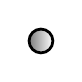
\begin{tikzpicture}\draw[left color=gray,line width=1pt] circle(1ex);\end{tikzpicture} & Mote
\end{tabular}
}
\end{center}
\end{column}
\begin{column}{0.5\textwidth}
\begin{center}
  \scalebox{0.6}{
  \begin{tikzpicture}[
    ack/.style={draw, rectangle, fill=orange!40, inner sep=0pt, outer sep=0pt},
    tx/.style={draw, rectangle, fill=blue!30,inner sep=0pt, outer sep=0pt},
    relay/.style={draw, rectangle, fill=green!30,inner sep=0pt, outer sep=0pt},
    rx/.style={draw, pattern=north west lines, pattern color=black!60, rectangle, inner sep=0pt, outer sep=0pt},
    arr/.style={help lines,black!70,<->},
    ]
    \draw[->,thick] (-0.1,0)--(6,0) node[right]{time};
    \draw[->,thick] (0,-0.1)--(0,4) node[above]{};

    \draw[dotted] (-0.1,0.5)--(6,0.5);
    \node[] at (-1.2, 1) {Gateway};
    \draw[] (-0.1,1)--(0.1,1);
    \draw[dotted] (-0.1,1.5)--(6,1.5);
    \node[] at (-1.2, 2) {Node 1};
    \draw[] (-0.1,2)--(0.1,2);
    \draw[dotted] (-0.1,2.5)--(6,2.5);
    \node[] at (-1.2, 3) {Node 2};
    \draw[] (-0.1,3)--(0.1,3);
    \draw[dotted] (-0.1,3.5)--(6,3.5);

    % Gateway
    \node () [rx, fit={(0.1,0.7) (5.9,1.3)}] {};
    \node () [relay, fit={(1.4,0.7) (1.6,1.3)}] {};
    \node () [relay, fit={(3.4,0.7) (3.6,1.3)}] {};
    \node () [relay, fit={(2.4,0.7) (2.6,1.3)}] {};
    % Relay
    \node () [tx, fit={(1.1,1.7) (1.4,2.3)}] {};
    \node () [rx, fit={(1.4,1.7) (1.6,2.3)}] {};
    \node () [tx, fit={(3.1,1.7) (3.4,2.3)}] {};
    \node () [rx, fit={(3.4,1.7) (3.6,2.3)}] {};
    \node () [tx, fit={(5.1,1.7) (5.4,2.3)}] {};
    % Node
    \node () [tx, fit={(2.1,2.7) (2.4,3.3)}] {};
    \node () [rx, fit={(2.4,2.7) (2.6,3.3)}] {};
    \node () [tx, fit={(5.1,2.7) (5.4,3.3)}] {};
  \end{tikzpicture}
  }
  % \caption{Collision between nodes}
  \scalebox{0.6}{
  \begin{tabular}{r@{ }l r@{ }l}
  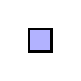
\begin{tikzpicture}\draw[fill=blue!30,line width=1pt] +(-4pt,-4pt) rectangle +(4pt,4pt);\end{tikzpicture} & Transmission 
    & \begin{tikzpicture}\draw[pattern=north west lines, pattern color=black!90,line width=1pt] +(-4pt,-4pt) rectangle +(4pt,4pt);\end{tikzpicture} & Reception
  \end{tabular}
  }
\end{center}
\end{column}
\end{columns}

\end{frame}

\begin{frame}{LoRaWAN}
\framesubtitle{Retransmission}
\begin{block}{}
{
  Quels sont les rêgles de retransmission des paquets un-ack ?
}
\end{block}
\begin{center}
\scalebox{0.6}{
\begin{tikzpicture}[
  ack/.style={draw, rectangle, fill=orange!40, inner sep=0pt, outer sep=0pt},
  tx/.style={draw, rectangle, fill=blue!30,inner sep=0pt, outer sep=0pt},
  relay/.style={draw, rectangle, fill=green!30,inner sep=0pt, outer sep=0pt},
  rx/.style={draw, pattern=north west lines, pattern color=black!60, rectangle, inner sep=0pt, outer sep=0pt},
  arr/.style={help lines,black!70,<->},
  ]
  \draw[->,thick] (-0.1,0)--(6,0) node[right]{time};
  \draw[->,thick] (0,-0.1)--(0,4) node[above]{};

  \draw[dotted] (-0.1,0.5)--(6,0.5);
  \node[] at (-1.2, 1) {Gateway};
  \draw[] (-0.1,1)--(0.1,1);
  \draw[dotted] (-0.1,1.5)--(6,1.5);
  \node[] at (-1.2, 2) {Node 1};
  \draw[] (-0.1,2)--(0.1,2);
  \draw[dotted] (-0.1,2.5)--(6,2.5);
  \node[] at (-1.2, 3) {Node 2};
  \draw[] (-0.1,3)--(0.1,3);
  \draw[dotted] (-0.1,3.5)--(6,3.5);

  \draw[->,very thick,dotted] (1.4,2)--(3.1,2);
  \draw[->,very thick,dotted] (1.4,3)--(5.1,3);

  % Gateway
  \node () [rx, fit={(0.1,0.7) (5.9,1.3)}] {};
  \node () [relay, fit={(3.4,0.7) (3.6,1.3)}] {};
  \node () [relay, fit={(5.4,0.7) (5.6,1.3)}] {};
  % Node 1
  \node () [tx, fit={(1.1,1.7) (1.4,2.3)}] {};
  \node () [tx, fit={(3.1,1.7) (3.4,2.3)}] {};
  \node () [rx, fit={(3.4,1.7) (3.6,2.3)}] {};
  % Node 2
  \node () [tx, fit={(1.1,2.7) (1.4,3.3)}] {};
  \node () [tx, fit={(5.1,2.7) (5.4,3.3)}] {};
  \node () [rx, fit={(5.4,2.7) (5.6,3.3)}] {};
\end{tikzpicture}
}
\end{center}
\begin{center}
\scalebox{0.6}{
\begin{tabular}{r@{ }l r@{ }l}
  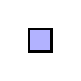
\begin{tikzpicture}\draw[fill=blue!30,line width=1pt] +(-4pt,-4pt) rectangle +(4pt,4pt);\end{tikzpicture} & Transmission 
    & \begin{tikzpicture}\draw[pattern=north west lines, pattern color=black!90,line width=1pt] +(-4pt,-4pt) rectangle +(4pt,4pt);\end{tikzpicture} & Reception
\end{tabular}
}
\end{center}

\end{frame}

\begin{frame}{LoRaWAN}
\framesubtitle{Multiplexing}
\begin{block}{}
{
  Comment éviter les collisions ?
}
\end{block}

\begin{columns}
  \begin{column}{0.5\textwidth}
    \makebox[\linewidth]{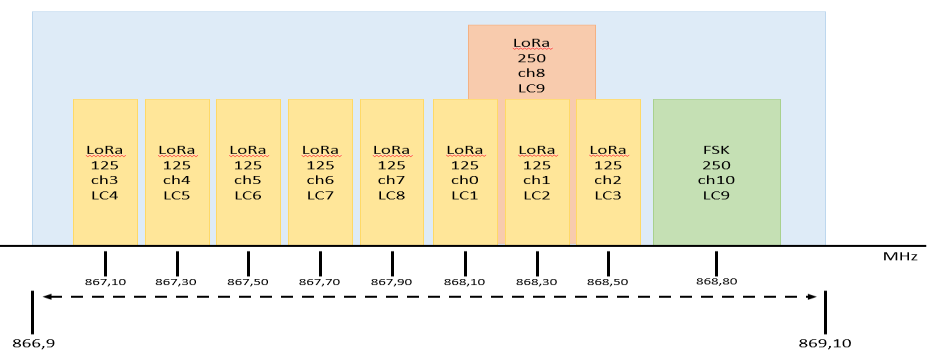
\includegraphics[page=1,width=0.45\paperwidth]{presentation.tex/fig/channels.png}}
  \end{column}
  \begin{column}{0.5\textwidth}
    \begin{center}
\scalebox{0.6}{
\begin{tikzpicture}[
  ack/.style={draw, rectangle, fill=orange!40, inner sep=0pt, outer sep=0pt},
  tx/.style={draw, rectangle, inner sep=0pt, outer sep=0pt},
  ch1/.style={fill=blue!30},
  ch2/.style={fill=red!30},
  ch3/.style={fill=green!30},
  rx/.style={draw, pattern=north west lines, pattern color=black!60, rectangle, inner sep=0pt, outer sep=0pt},
  arr/.style={help lines,black!70,<->},
  ]
  \draw[->,thick] (-0.1,0)--(6,0) node[right]{time};
  \draw[->,thick] (0,-0.1)--(0,5) node[above]{};

  \draw[dotted] (-0.1,0.5)--(6,0.5);
  \node[] at (-1.2, 1) {Gateway};
  \draw[] (-0.1,1)--(0.1,1);
  \draw[dotted] (-0.1,1.5)--(6,1.5);
  \node[] at (-1.2, 2) {$Ch_{1}$};
  \draw[] (-0.1,2)--(0.1,2);
  \draw[dotted] (-0.1,2.5)--(6,2.5);
  \node[] at (-1.2, 3) {$Ch_{2}$};
  \draw[] (-0.1,3)--(0.1,3);
  \draw[dotted] (-0.1,3.5)--(6,3.5);
  \node[] at (-1.2, 4) {$Ch_{3}$};
  \draw[] (-0.1,4)--(0.1,4);
  \draw[dotted] (-0.1,4.5)--(6,4.5);

  % Gateway
  \node () [rx, fit={(0.1,0.7) (5.9,1.3)}] {};
  \node () [tx, ch1, fit={(1.4,0.7) (1.6,1.3)}] {};
  \node () [tx, ch2, fit={(2.4,0.7) (2.6,1.3)}] {};
  \node () [tx, ch3, fit={(3.4,0.7) (3.6,1.3)}] {};
  % Ch 1
  \node () [tx, ch1, fit={(1.1,1.7) (1.4,2.3)}] {};
  \node () [rx, fit={(1.4,1.7) (1.6,2.3)}] {};
  % Ch 2
  \node () [tx, ch2, fit={(2.1,2.7) (2.4,3.3)}] {};
  \node () [rx, fit={(2.4,2.7) (2.6,3.3)}] {};
  % Ch 3
  \node () [tx, ch3, fit={(3.1,3.7) (3.4,4.3)}] {};
  \node () [rx, fit={(3.4,3.7) (3.6,4.3)}] {};
\end{tikzpicture}
}
\end{center}
\begin{center}
\scalebox{0.6}{
\begin{tabular}{r@{ }l r@{ }l}
  \begin{tikzpicture}\draw[pattern=north west lines, pattern color=black!90,line width=1pt] +(-4pt,-4pt) rectangle +(4pt,4pt);\end{tikzpicture} & Reception
    & 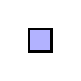
\begin{tikzpicture}\draw[fill=blue!30,line width=1pt] +(-4pt,-4pt) rectangle +(4pt,4pt);\end{tikzpicture} & Channel 1 \\
  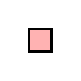
\begin{tikzpicture}\draw[fill=red!30,line width=1pt] +(-4pt,-4pt) rectangle +(4pt,4pt);\end{tikzpicture} & Channel 2
    & 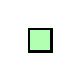
\begin{tikzpicture}\draw[fill=green!30,line width=1pt] +(-4pt,-4pt) rectangle +(4pt,4pt);\end{tikzpicture} & Channel 3
\end{tabular}
}
\end{center}

  \end{column}
\end{columns}

\end{frame}

\begin{frame}{LoRaWAN}
\framesubtitle{Adaptive Data Rate}
\begin{block}{}
{
  Comment étendre la portée ?
}
\end{block}
\begin{columns}
\begin{column}{0.5\textwidth}
\begin{center}
\scalebox{0.8}{
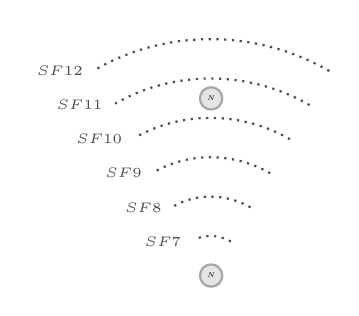
\begin{tikzpicture}[
    state/.style={circle, thick,draw=gray!70,fill=gray!20,text=black,scale=0.5},
]
\tikzset{
  pics/carc/.style args={#1:#2:#3:#4}{
    code={
      \draw[pic actions] (#1:#3) arc(#1:#2:#3) node[at end,left, black!70] {\tiny #4};
    }
  }
}
\begin{scope}[shorten >=1pt,auto,node distance=4.5cm]
  \node[state]         (A) [] {\tiny $N$};
  \node[state]         (B) [below of=A]       {\tiny $N$};
  \draw[black!70, dotted, thick] (B) pic{carc=60:120:0.5cm:$SF7$}
    pic{carc=60:120:1cm:$SF8$} pic{carc=60:120:1.5cm:$SF9$}
    pic{carc=60:120:2cm:$SF10$} pic{carc=60:120:2.5cm:$SF11$}
    pic{carc=60:120:3cm:$SF12$};
\end{scope}
\end{tikzpicture}
}
\end{center}
\end{column}
\begin{column}{0.5\textwidth}
\begin{center}
\scalebox{0.6}{
\begin{tikzpicture}[
  ack/.style={draw, rectangle, fill=orange!40, inner sep=0pt, outer sep=0pt},
  tx/.style={draw, rectangle, fill=blue!30,inner sep=0pt, outer sep=0pt},
  relay/.style={draw, rectangle, fill=green!30,inner sep=0pt, outer sep=0pt},
  rx/.style={draw, pattern=north west lines, pattern color=black!60, rectangle, inner sep=0pt, outer sep=0pt},
  arr/.style={help lines,black!70,<->},
  ]
  \draw[->,thick] (-0.1,0)--(6,0) node[right]{time};
  \draw[->,thick] (0,-0.1)--(0,6) node[above]{};

  \draw[dotted] (-0.1,0.5)--(6,0.5);
  \node[] at (-1.2, 1) {Gateway};
  \draw[] (-0.1,1)--(0.1,1);
  \draw[dotted] (-0.1,1.5)--(6,1.5);
  \node[] at (-1.2, 2) {$SF_{7}$};
  \draw[] (-0.1,2)--(0.1,2);
  \draw[dotted] (-0.1,2.5)--(6,2.5);
  \node[] at (-1.2, 3) {$SF_{8}$};
  \draw[] (-0.1,3)--(0.1,3);
  \draw[dotted] (-0.1,3.5)--(6,3.5);
  \node[] at (-1.2, 4) {$...$};
  \draw[] (-0.1,4)--(0.1,4);
  \draw[dotted] (-0.1,4.5)--(6,4.5);
  \node[] at (-1.2, 5) {$SF_{11}$};
  \draw[] (-0.1,5)--(0.1,5);
  \draw[dotted] (-0.1,5.5)--(6,5.5);

  \path (1.3,2) edge[->,dotted,very thick,bend left,black!70] (2.1,2.7);
  \path (2.2,3) edge[->,dotted,very thick,bend left,black!70] (5.1,4.7);

  % Gateway
  \node () [rx, fit={(0.1,0.7) (5.9,1.3)}] {};
  \node () [relay, fit={(5.4,0.7) (5.6,1.3)}] {};
  % SF7
  \node () [tx, fit={(1.1,1.7) (1.4,2.3)}] {};
  % SF8
  \node () [tx, fit={(2.1,2.7) (2.4,3.3)}] {};
  % ...
  % SF11
  \node () [tx, fit={(5.1,4.7) (5.4,5.3)}] {};
  \node () [rx, fit={(5.4,4.7) (5.6,5.3)}] {};
\end{tikzpicture}
}
% \caption{Collision between nodes}
\scalebox{0.6}{
\begin{tabular}{r@{ }l r@{ }l}
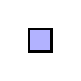
\begin{tikzpicture}\draw[fill=blue!30,line width=1pt] +(-4pt,-4pt) rectangle +(4pt,4pt);\end{tikzpicture} & Transmission 
  & \begin{tikzpicture}\draw[pattern=north west lines, pattern color=black!90,line width=1pt] +(-4pt,-4pt) rectangle +(4pt,4pt);\end{tikzpicture} & Reception
\end{tabular}
}
\end{center}
\end{column}
\end{columns}

\end{frame}

\begin{frame}{LoRaWAN}
\framesubtitle{Pourquoi ce succès ?}
\begin{itemize}
  \item LoRaWAN est open source contrairement à ses concurrents
  \begin{itemize}
    \item Implémentations indépendante de Semtech
  \end{itemize}
  \item Possible de créer son réseau privé  
  \item Possible de créer son propre protocol basé sur LoRa PHY
  \item The Things Network
  \begin{itemize}
    \item Réseau publique LoRaWAN crowdfunder
    \item Offrir sa gateway à d'autres utilisateurs
  \end{itemize}
\end{itemize}
\end{frame}

\begin{frame}{LoRaWAN}
\framesubtitle{Aller plus loin}
\begin{columns}
  \begin{column}{0.5\textwidth}
    
\begin{itemize}
  \item Limitation pour le downlink
  \begin{itemize}
    \item Pas possible d'utiliser les ED comme des actuateurs
    \item Class B et C
  \end{itemize}
  \item Création de réseau multihop
  \begin{itemize}
    \item Problème avec la consommation
  \end{itemize}
  \item Intégration à 6LoWPAN/6TiSCH
  \begin{itemize}
    \item IPv6 sur des microcontrolleurs
    \item Routing entre noeuds
    \item Basse consommation
  \end{itemize}
  \item LoRa 2.4GHz, LoRaSAT
\end{itemize}
\end{column}
\begin{column}{0.5\textwidth}
\begin{center}
\scalebox{0.9}{
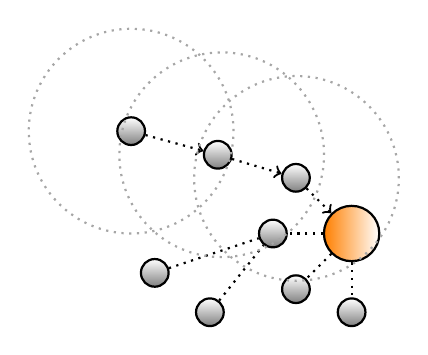
\begin{tikzpicture}[auto, thick]
  \tikzstyle{motes}=[draw,circle,bottom color= gray, top color= white,minimum width=10pt]
  \tikzstyle{gateways}=[draw,circle, left color= orange,minimum width=20pt]
  % Place super peers and connect them
  \foreach \place/\name in {{(0,0)/a}}
    \node[gateways] (\name) at \place {};
  \node[motes] (a4) at (-1.7, 1) {};
  \node[motes] (a5) at (-2.8, 1.3) {};
  \node[motes] (a7) at (-2.5, -0.5) {};
  \node[motes] (a8) at (-1.8, -1) {};
  \foreach \pos/\i in {below left of/1, below of/2, left of/3}
    \node[motes, \pos =a ] (a\i) {};
  \foreach \speer/\peer in {a/a1,a/a2,a/a3,a7/a3,a8/a3}
    \path[dotted] (\speer) edge (\peer);

  \node[motes, above left of=a ] (a6) {};
  \path[dotted,->] (a5) edge (a4);
  \path[dotted,->] (a4) edge (a6);
  \path[dotted,->] (a6) edge (a);
  \draw[dotted,draw={black},color=gray!70] (-2.8,1.3) circle (1.3cm);
  \draw[dotted,draw={black},color=gray!70] (-1.65,1) circle (1.3cm);
  \draw[dotted,draw={black},color=gray!70] (-0.7,0.7) circle (1.3cm);
\end{tikzpicture}
}
\end{center}
\begin{center}
\scalebox{0.5}{%
\begin{tabular}{r@{: }l r@{: }l}

\begin{tikzpicture}\draw[left color=orange,line width=1pt]
    circle(1ex);\end{tikzpicture} & Gateway & 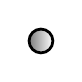
\begin{tikzpicture}\draw[left color=gray,line width=1pt] circle(1ex);\end{tikzpicture} & Mote
\end{tabular}
}
\end{center}
\end{column}
\end{columns}
\end{frame}

\begin{frame}{LoRaWAN}
\framesubtitle{SDR}
\begin{columns}
  \begin{column}{0.5\textwidth}
  \begin{itemize}
    \item Observable avec un RTL-SDR peu cher
    \item 500kHz - 1766 MHz
    \item Tentative de reverse du protocol disponible
    \item GNU Radio
  \end{itemize}
  \end{column}
  \begin{column}{0.5\textwidth}
   \begin{center}
    \makebox[\linewidth]{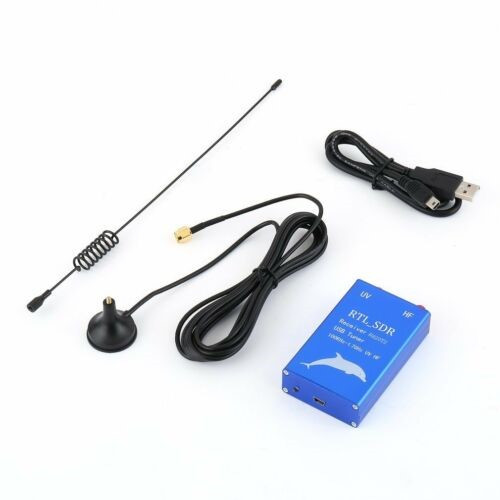
\includegraphics[page=1,width=0.50\paperwidth]{presentation.tex/fig/sdr.jpg}}
  \end{center}
  \end{column}
\end{columns}

\end{frame}


